Sofía arma cuadrados con fósforos. En la siguiente imagen, hay tres figuras que Sofía armó:

\begin{minipage}{0.4\linewidth}
    \begin{figure}[H]
        \centering
        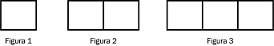
\includegraphics[width=0.9\textwidth]{../images/9b2788ac343174f7bbf340e98582d00a42c4804d}
    \end{figure}
\end{minipage}\hfill
\begin{minipage}{0.6\linewidth}
    Sofía observa esta secuencia de figuras y dice:
    Si sigo armando cuadrados según esta secuencia, al terminar de armar la Figura 20, habré utilizado menos de 640 fósforos.\\
    \textbf{¿Es correcto lo que dice Sofía? ¿Por qué?}\\
\end{minipage}

\begin{solutionbox}{5.5cm}
    La regla de recurrencia para la serie de fósforos es:
    \[a_n=3(n-1)+4\]
    Calculando $a_{19}$
    \[a_{20}=3(20-1)+4=61\]
    Utilizando la suma de los términos de una serie:
    \[s_{20}=\dfrac{20(4+61)}{2}=650\]
    Por lo tanto, no es correcto lo que dice Sofía, ya que: tendrá 650 canicas al cabo de 30 días.
\end{solutionbox}